% Created 2020-11-19 czw 08:34
% Intended LaTeX compiler: pdflatex
\documentclass[11pt]{article}
\usepackage[utf8]{inputenc}
\usepackage[T1]{fontenc}
\usepackage{graphicx}
\usepackage{grffile}
\usepackage{longtable}
\usepackage{wrapfig}
\usepackage{rotating}
\usepackage[normalem]{ulem}
\usepackage{amsmath}
\usepackage{textcomp}
\usepackage{amssymb}
\usepackage{capt-of}
\usepackage{hyperref}
\renewcommand*{\contentsname}{Spis Treści}
\usepackage[margin=3cm]{geometry}
\hypersetup{colorlinks=true,linkcolor=blue}
\usepackage{fancyhdr}
\usepackage{graphicx}
\graphicspath{ {/home/thisconnect/pwsz/} }
\pagestyle{fancyplain}
\chead{Router IP}
\lhead{\includegraphics{pusb.png}}
\rhead{}
\cfoot{}
\lfoot{}
\rfoot{Patryk Kaniewski \linebreak GNU GPLv3}
\author{Patryk Kaniewski}
\date{\today}
\title{Router IP \\
Patryk Kaniewski}
\hypersetup{
 pdfauthor={Patryk Kaniewski},
 pdftitle={Router IP \\
Patryk Kaniewski},
 pdfkeywords={},
 pdfsubject={},
 pdfcreator={Emacs 27.1 (Org mode 9.3)}, 
 pdflang={Polish}}
\begin{document}

\begin{titlepage}
\begin{center}
{\Huge Router IP \par}
\vspace{2cm}
{\Large Patryk Kaniewski \par
}\vspace{2cm}
{\large 2020-10-22}
\end{center}
\end{titlepage}
\setcounter{tocdepth}{2}
\tableofcontents \clearpage

\section{Grupa wykonująca zadanie}
\label{sec:org8edc83e}
\begin{itemize}
\item Patryk Kaniewski
\item Jakub Caban
\item Dominik Gandziarek
\end{itemize}

\section{Wstęp}
\label{sec:org568ddb8}
\subsection{Cel ćwiczenia}
\label{sec:org3b9c606}
Celem ćwiczenia jest pokazanie w jaki sposób NAT (Network Adress Translation) ukrywa strukturę sieci wewnetrznej
\subsection{Schemat ćwiczenia}
\label{sec:org16e6f6f}
\begin{center}
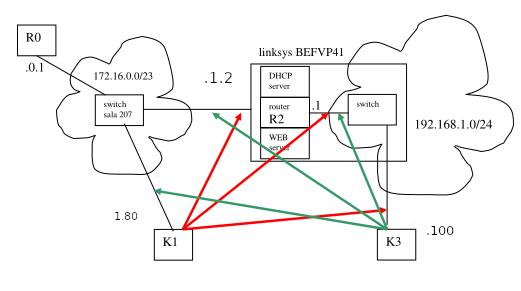
\includegraphics[width=.9\linewidth]{./schemat.png}
\end{center}
\subsection{Wymagany sprzęt}
\label{sec:orgd751965}
\begin{itemize}
\item Router z możliwościa wyłaczenia NAT (np Linksys BEFVP41)
\item 2 Komputery osobiste
\item skrętka komputerowa UTP zakonczona 8PC8 (np. cat5e)
\end{itemize}

\subsection{Plan ćwiczenia}
\label{sec:org1cd9d97}
\begin{enumerate}
\item Podłączenie routera i komputerów wg. schematu
\item Właczenie i zalogowanie sie na router i komputery (może być potrzebne konto administratora)
\item Badanie zachowania się sieci NAT (np. ping K1<->R1<->K3)
\item Wyłaczenie sieci NAT na routerze (w BEFVP41 NAT Setup->Advanced Routing->Dynamic Routing->NAT->Disabled)
\item Ustawienie recznej konfiguracji R1 (zmiana domyślnej bramy na WAN routera)
\end{enumerate}


\section{Ćwiczenie}
\label{sec:org39bd9f4}
\subsection{Wstępna konfiguracja}
\label{sec:org7daec33}
\subsubsection{K1}
\label{sec:orgbe5b300}
\begin{verbatim}
Ethernet adapter Ethernet:

   Connection-specific DNS Suffix  . : pwsz.pk
   Link-local IPv6 Address . . . . . : fe80::1cb5:9d48:9e1b:f847%11
   IPv4 Address. . . . . . . . . . . : 172.16.1.80
   Subnet Mask . . . . . . . . . . . : 255.255.254.0
   Default Gateway . . . . . . . . . : 172.16.0.1~
\end{verbatim}
\subsubsection{K3}
\label{sec:org849465a}
\begin{verbatim}
Windows IP Configuration


Ethernet adapter Ethernet:

   Connection-specific DNS Suffix  . : pwsz.pk
   Link-local IPv6 Address . . . . . : fe80::dc70:7154:4ecd:c188%4
   IPv4 Address. . . . . . . . . . . : 192.168.1.100
   Subnet Mask . . . . . . . . . . . : 255.255.255.0
   Default Gateway . . . . . . . . . : 192.168.1.1
\end{verbatim}
\subsubsection{R1}
\label{sec:org8507a75}
\begin{center}
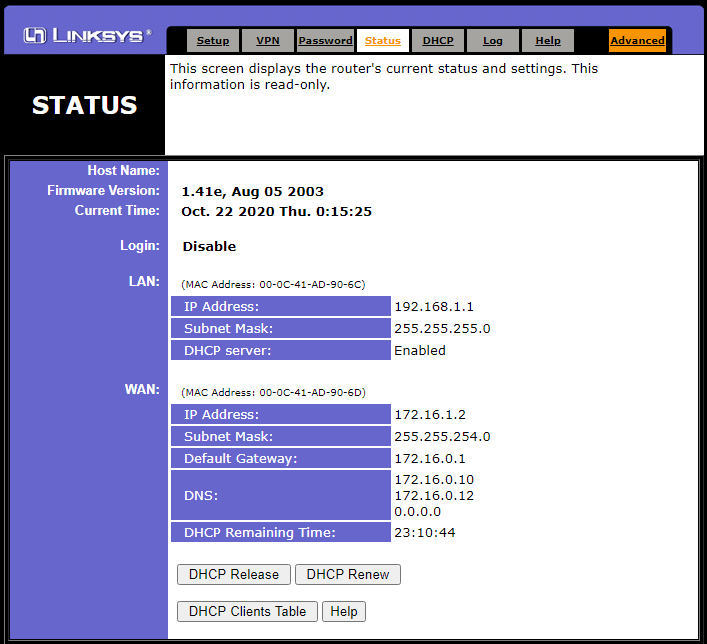
\includegraphics[width=.9\linewidth]{./router_interfejsy.png}
\end{center}
\subsection{Badanie zachowania NAT}
\label{sec:org11f24db}
\subsubsection{K3 -> K1}
\label{sec:org43249dc}
Pingowanie z sieci NAT do sieci zewnętrznej jest normalnym zachowaniem które można zaobserować podczas poprawnego działania wiekszości połaczeń internetowych
\begin{verbatim}
Pinging 172.16.1.80 with 32 bytes of data:
Reply from 172.16.1.80: bytes=32 time=2ms TTL=128
Reply from 172.16.1.80: bytes=32 time=2ms TTL=128
Reply from 172.16.1.80: bytes=32 time=3ms TTL=128
Reply from 172.16.1.80: bytes=32 time=2ms TTL=128

Ping statistics for 172.16.1.80:
    Packets: Sent = 4, Received = 4, Lost = 0 (0% loss),
Approximate round trip times in milli-seconds:
    Minimum = 2ms, Maximum = 3ms, Average = 2ms
\end{verbatim}
Jak widać adresem źrodłowym jest adress zewnętrzny routera IP a nie K3
\begin{center}
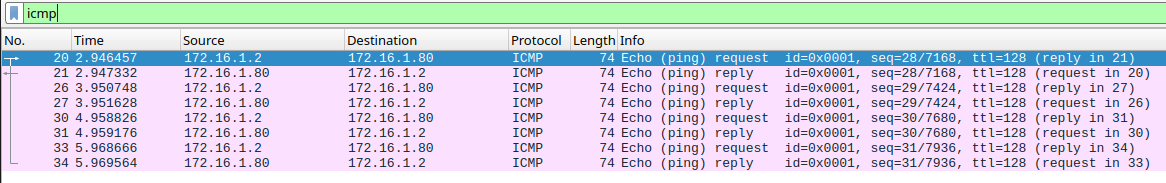
\includegraphics[width=.9\linewidth]{./K1/przed/k1_pingk3dok1.png}
\end{center}

\subsubsection{K1 -> K3}
\label{sec:org945542a}
NAT nie pozwala pingować wewnętrznych zasobów sieciowych
\begin{verbatim}
Pinging 192.168.1.100 with 32 bytes of data:
Request timed out.
Request timed out.
Request timed out.
Request timed out.

Ping statistics for 192.168.1.100:
    Packets: Sent = 4, Received = 0, Lost = 4 (100% loss),
\end{verbatim}
\subsubsection{K1-> R2(LAN)}
\label{sec:org2559969}
Jak iż nie widzimy wewnętrznej sieci, pingi na adress wewnętrzny również sa odrzucane
\begin{verbatim}
Pinging 192.168.1.1 with 32 bytes of data:
Request timed out.
Request timed out.
Request timed out.
Request timed out.

Ping statistics for 192.168.1.1:
    Packets: Sent = 4, Received = 0, Lost = 4 (100% loss),
\end{verbatim}
\subsection{Wyłączenie NAT}
\label{sec:org3659aa0}
Należy wyłaczyć router NAT na routerze.
Dla Linksys NAT Setup->Advanced Routing->Dynamic Routing->NAT->Disabled.
\subsubsection{K1}
\label{sec:org89c410d}
Aby umożliwić dwustronna komunikacje musimy ręcznie ustawić interfejs sieciowy na K1.

Należy ustawic bramę domyślna na adres WAN R2 (w naszym przypadku 172.16.1.2).
\begin{verbatim}
Windows IP Configuration


Ethernet adapter Ethernet:

   Connection-specific DNS Suffix  . : 
   Link-local IPv6 Address . . . . . : fe80::1cb5:9d48:9e1b:f847%11
   IPv4 Address. . . . . . . . . . . : 172.16.1.80
   Subnet Mask . . . . . . . . . . . : 255.255.254.0
   Default Gateway . . . . . . . . . : 172.16.1.2
\end{verbatim}
\subsection{Badanie zachowania Routera bez NAT}
\label{sec:org22453dd}
\subsubsection{K3->K1}
\label{sec:orgc965f0d}
Połączenie z sieci wewnętrznej na zewnątrz nadal jest utrzymane.
\begin{verbatim}
Pinging 172.16.1.80 with 32 bytes of data:
Reply from 172.16.1.80: bytes=32 time=2ms TTL=127
Reply from 172.16.1.80: bytes=32 time=2ms TTL=127
Reply from 172.16.1.80: bytes=32 time=2ms TTL=127
Reply from 172.16.1.80: bytes=32 time=2ms TTL=127

Ping statistics for 172.16.1.80:
    Packets: Sent = 4, Received = 4, Lost = 0 (0% loss),
Approximate round trip times in milli-seconds:
    Minimum = 2ms, Maximum = 2ms, Average = 2ms
\end{verbatim}
\subsubsection{K1->K3}
\label{sec:orgac8ecbb}
Po wyłączeniu translacji adresów, mamy pełen dostęp do sieci wewnętznej 192.168.1.0/24.
\begin{verbatim}
Pinging 192.168.1.100 with 32 bytes of data:
Reply from 192.168.1.100: bytes=32 time=2ms TTL=127
Reply from 192.168.1.100: bytes=32 time=2ms TTL=127
Reply from 192.168.1.100: bytes=32 time=3ms TTL=127
Reply from 192.168.1.100: bytes=32 time=3ms TTL=127

Ping statistics for 192.168.1.100:
    Packets: Sent = 4, Received = 4, Lost = 0 (0% loss),
Approximate round trip times in milli-seconds:
    Minimum = 2ms, Maximum = 3ms, Average = 2ms
\end{verbatim}
Możemy zaobserwować jawność adresów obydwu maszyn.
\begin{center}
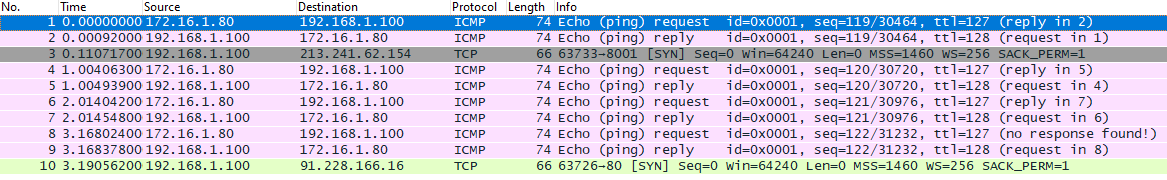
\includegraphics[width=.9\linewidth]{./K3/ping_z_K1.png}
\end{center}
\subsubsection{K1->R2}
\label{sec:orgfaf5acc}
Po usunięciu blokady na pingi na routerze (patrz \ref{sec:org5d77367}). Możemy pingować wszystkie interfejsy routera z sieci wewnętrznej.
\begin{verbatim}
Pinging 192.168.1.1 with 32 bytes of data:
Reply from 192.168.1.1: bytes=32 time=1ms TTL=150
Reply from 192.168.1.1: bytes=32 time=1ms TTL=150
Reply from 192.168.1.1: bytes=32 time=1ms TTL=150
Reply from 192.168.1.1: bytes=32 time=1ms TTL=150

Ping statistics for 192.168.1.1:
    Packets: Sent = 4, Received = 4, Lost = 0 (0% loss),
Approximate round trip times in milli-seconds:
    Minimum = 1ms, Maximum = 1ms, Average = 1ms
\end{verbatim}
\begin{verbatim}
Pinging 172.16.1.2 with 32 bytes of data:
Reply from 172.16.1.2: bytes=32 time=1ms TTL=150
Reply from 172.16.1.2: bytes=32 time=1ms TTL=150
Reply from 172.16.1.2: bytes=32 time=1ms TTL=150
Reply from 172.16.1.2: bytes=32 time=1ms TTL=150

Ping statistics for 172.16.1.2:
    Packets: Sent = 4, Received = 4, Lost = 0 (0% loss),
Approximate round trip times in milli-seconds:
    Minimum = 1ms, Maximum = 1ms, Average = 1ms
\end{verbatim}
\section{Wnioski}
\label{sec:orgb11093f}
\subsection{Działanie NAT}
\label{sec:org9169d66}
NAT maskuje wszystkie urządzenia które sie za nim znajdują. Utrudnia on zewnętrzny dostęp do wewnętrznych zasobów sieciowych.
Wewnętrzne urządzenia wychodząc na sieci zewnętrzne sa ukrywane (router NAT nadpisuje w pakiecie IP pole source adress).
\subsection{Napotkane problemy}
\label{sec:org5d77367}
Domyślnie router Linksys blokuje zewnętrzne pingi.

Tą opcje można wyłaczyć w Filters-> Block WAN Request
\begin{center}
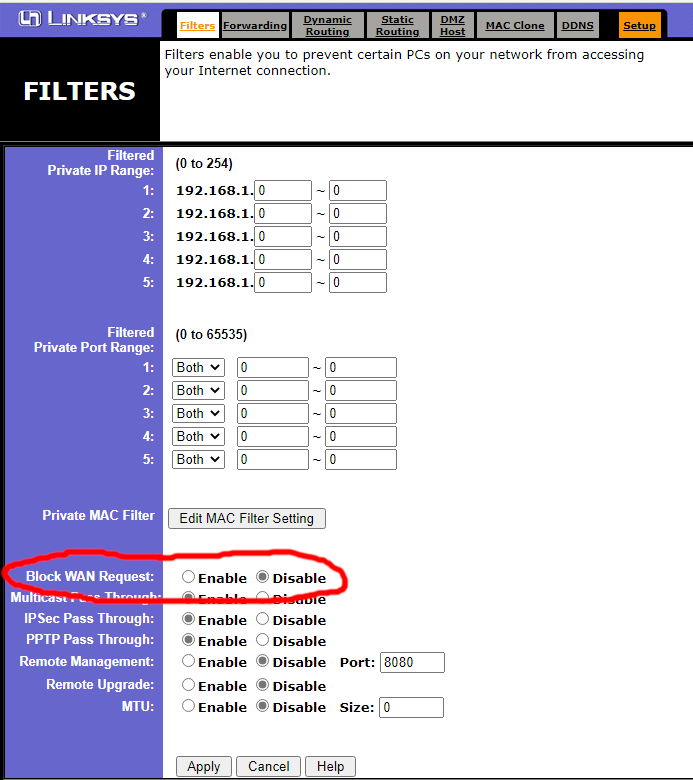
\includegraphics[width=.9\linewidth]{./K3/wylaczenie_opcji_na_routerze_block_wan.png}
\end{center}
\end{document}
